\documentclass[journal]{IEEEtran}
\usepackage{amsmath,amsfonts}
% \usepackage{algorithmic}
\usepackage{algorithm}
\usepackage{algpseudocode} % For more flexible 
\usepackage{array}
% \usepackage[caption=false,font=normalsize,labelfont=sf,textfont=sf]{subfig}
\usepackage[]{subfig}
\usepackage{textcomp}
\usepackage{stfloats}
\usepackage{url}
\usepackage{verbatim}
\usepackage{graphicx}
% \usepackage{booktabs} % For professional-quality tables
\usepackage{cite}

\usepackage{makecell}   % 支持更灵活的单元格对齐和内容换行
\usepackage{multirow}
\usepackage{pifont}
\hyphenation{op-tical net-works semi-conduc-tor IEEE-Xplore}
% updated with editorial comments 8/9/2021


% -------------------------允许算法跨页-------------
\makeatletter
\newenvironment{breakablealgorithm}
  {% \begin{breakablealgorithm}
   \begin{center}
     \refstepcounter{algorithm}% New algorithm
     \hrule height.8pt depth0pt \kern2pt% \@fs@pre for \@fs@ruled
     \renewcommand{\caption}[2][\relax]{% Make a new \caption
       {\raggedright\textbf{\ALG@name~\thealgorithm} ##2\par}%
       \ifx\relax##1\relax % #1 is \relax
         \addcontentsline{loa}{algorithm}{\protect\numberline{\thealgorithm}##2}%
       \else % #1 is not \relax
         \addcontentsline{loa}{algorithm}{\protect\numberline{\thealgorithm}##1}%
       \fi
       \kern2pt\hrule\kern2pt
     }
  }{% \end{breakablealgorithm}
     \kern2pt\hrule\relax% \@fs@post for \@fs@ruled
   \end{center}
  }
\makeatother

% \usepackage{subcaption} % 支持子图功能
% \usepackage{subfigure}

% \usepackage{float} % 使 [H] 参数生效

\begin{document}

\title{Semi-Asynchronous Energy-Efficient Federated Prototype Learning for Client-Edge-Cloud Architectures}

% \author{IEEE Publication Technology,~\IEEEmembership{Staff,~IEEE,}

% The paper headers
% \markboth{Journal of \LaTeX\ Class Files,~Vol.~14, No.~8, August~2021}%
% {Shell \MakeLowercase{\textit{et al.}}: A Sample Article Using IEEEtran.cls for IEEE Journals}

% \IEEEpubid{0000--0000/00\$00.00~\copyright~2021 IEEE}
% Remember, if you use this you must call \IEEEpubidadjcol in the second
% column for its text to clear the IEEEpubid mark.

\maketitle

\begin{abstract}

\end{abstract}

\begin{IEEEkeywords}
  Federated Prototype Learning, Hierarchical Architecture, Heterogeneous Models, Asynchronous Communication, Energy Efficiency
\end{IEEEkeywords}

\section{Introduction}
\IEEEPARstart{C}{urrently}, academia is exploring the vision of Industry 5.0 \cite{zeb2024towards_industry5.0, leng2024unlocking_industry5.0}, which focuses on sustainability, resiliency, and human-centered values. In this context, the core concept of Industry 5.0 is achieving customized production with zero waste and minimized cost through advanced technologies such as the Industrial Internet of Things (IIoT) \cite{zeb2024towards_industry5.0,10440434}, where AI technologies support various tasks, such as pattern recognition and decision making, by processing large amounts of real-time data. This drives industrial processes intelligence, significantly improving productivity \cite{liu2024federated_sensors, de2024spatio_agriculture}. Although the conventional centralized learning paradigm, such as cloud computing, provides benefits, including resource sharing and significant scalability, they simultaneously pose issues related to data privacy and security \cite{boobalan2022fusion}. Furthermore, cloud computing encounters difficulties in fulfilling the immediate processing demands of IIoT data because of elevated transmission costs and delays, which in turn have a direct influence on energy consumption and carbon emissions.

%, while addressing global challenges such as environmental protection and social stability \cite{10440434}.  , especially when aggregating user data artificial intelligence, the Internet of Things (IoT), and big data. T is a crucial component of Industry 5.0 


To improve data protection and computation efficiency, Google first introduced federated learning (FL) in 2016 \cite{fedavg_google} by combining cloud and edge computing for distributed learning, aggregating a model in the cloud. Recently, it has been widely applied in IIoT applications, such as security protection \cite{salim2024fl_securityguard} and intrusion detection \cite{rashid2023federated_invasion}. 

In FL, computation shifts from the cloud center to the edge, reducing the high-energy consumption of cloud servers. However, the large number of edge devices running for extended periods still results in significant and difficult-to-estimate energy consumption. In the study \cite{liu_hierarchical_2023}, the time and energy consumed for transmitting model parameters far exceed that of the computation. Therefore, in order to further reduce energy consumption and carbon emissions without compromising service quality, an efficient communication method combined with energy-efficient computation is urgently needed.

To address communication challenges, various architectures have been explored. First, the cloud-edge-device hierarchical architecture \cite{abdellatif2022communication_hierarchical,zhou2023hierarchical} balances low latency and efficient learning, effectively resolving the trade-off between communication efficiency and training performance in traditional two-layer systems \cite{liu_hierarchical_2023}. Moreover, to eliminate server communication bottlenecks, decentralized federated learning (DFL) architectures \cite{kalra2023decentralized,al2023decentralized_D2D} enable peer-to-peer collaboration among multiple devices, optimizing two-hop transmission in layered frameworks while further enhancing privacy protection. A large number of energy-efficient algorithms for FL have been proposed. \cite{chen_eefl_2023} and \cite{rashid2023federated_invasion} utilize DVFS (dynamic voltage and frequency scaling) technology to adjust device operating frequency, thereby reducing the high energy consumption caused by high-frequency operations. Lowering the model precision and quantizing can also achieve energy savings, as demonstrated by approaches such as \cite{de2023hed_quantize,chen2022energy_quantize}. 

However, the introduced architectures still face significant challenges. The global synchronization mechanism struggles to achieve efficient aggregation, particularly in scenarios with heterogeneous device performance and complex communication environments. Furthermore, most architectures \cite{luo2024communication_CEC,wu2023hiflash_CEC} are only suitable for homogeneous models and lack adequate adaptability to heterogeneous model settings. Most existing energy-saving methods rely on static estimations of execution time. However, training time is significantly influenced by factors such as device architecture and workload variations. Theoretical calculations of optimal frequency often results in suboptimal energy efficiency. It is imperative to design architectures capable of balancing model accuracy and energy efficiency in complex scenarios with heterogeneous models and data distributions.

Our proposed method is based on federated prototype learning, which requires clients to upload data distribution information while ensuring privacy protection, effectively addressing data imbalance and model heterogeneity issues. The hierarchical architecture ensures convergence \cite{liu_hierarchical_2023} and significantly reduces the wireless communication overhead. An asynchronous global aggregation approach is proposed, avoiding the time delay caused by global synchronization, thereby reducing the system's energy consumption. Synchronous model aggregation is performed at the edge level, and DVFS technology is introduced to further enhance energy efficiency. 

Specifically, the contributions of this paper are as follows:
\begin{enumerate}
    \item We collect privacy-independent data distribution information to train a global classifier on the cloud, which guides local client training, thereby enhancing prototype aggregation effectiveness and model accuracy.  
    \item We replace global synchronous aggregation with semi-asynchronous aggregation, which achieves the same model accuracy as synchronous aggregation without the need to account for complex staleness issues.  
    \item During the training process, we synchronize client first-round training time at the edge level and utilize DVFS to dynamically scale frequencies, achieving efficient energy savings.  
    \item Compared to popular heterogeneous federated learning methods, experimental results demonstrate that the proposed approach not only improves model accuracy but also significantly enhances energy efficiency.
\end{enumerate} 


\section{Related Work}
% \subsection{Heterogeneous Federated Learning}
% \subsection{Federated Prototype Learning}
With the advancement of digitalization and intelligent technologies, a vast array of IoT devices are dispersed globally, collecting valuable and privacy-sensitive data. Federated Learning (FL) has emerged as a promising paradigm, enabling the training of large models on these edge devices while preserving data privacy. However, traditional FL methods, such as FedAvg\cite{fedavg_google}, face significant performance degradation and increased communication costs when confronted with statistic, model, and device heterogeneity in practical scenarios. Heterogeneous Federated Learning (HtFL)\cite{tan2022fedproto} has been proposed to address these issues, allowing devices to maintain their privacy without sharing private model parameters and accommodating differences in model architectures and data distributions.

Some methods adopt a partially heterogeneous approach, allowing different underlying architectures but sharing the top layer. FedGH\cite{yi2023fedgh} aggregates local feature vectors from clients to train a shared generalized global prediction head, but it overlooks the differences in local features of clients. FedGen\cite{zhu2021data} trains a global representation generator, primarily used to introduce global knowledge to small classifiers. These partially heterogeneous methods allow clients to access limited global knowledge through a smaller global part, leading to performance degradation.

Another set of HtFL methods is fully heterogeneous, achieving this through advanced global knowledge sharing. A classic approach for global knowledge sharing is knowledge distillation. FedDistill\cite{jeong2018communication} shares the model's output logits to train the global model. FedKD\cite{wu2022communication} employs mutual distillation between an auxiliary global model and client models to share knowledge, reducing communication costs. FedKTL\cite{zhang2024upload} transfers knowledge from a pre-trained generator on the server to client models, while sharing task-specific knowledge among clients.
Another popular approach is sharing compact class representatives, such as prototypes. FedProto\cite{tan2022fedproto} introduces prototypes into federated learning, significantly reducing communication costs, but it still performs suboptimally under heterogeneous data conditions. FedTGP\cite{zhang2024fedtgp} uses contrastive learning to increase the spacing between globally aggregated prototypes, forming more distinct class intervals. However, the spacing between global prototypes continues to increase, and convergence cannot be guaranteed.

Addressing the energy constraints characteristic of IoT devices, Dynamic Voltage and Frequency Scaling (DVFS) emerges as a pivotal technique for conserving CPU and GPU energy through the modulation of voltage and frequency levels. This technique finds extensive application in AIoT-related research. You et al. \cite{you2023zeus} introduced a learning-based methodology for DVFS prediction, yielding prediction results of considerable accuracy. Dai et al.\cite{dai2024energy} proposed a dynamic approach to network exit based on the complexity of samples, coupled with corresponding adjustments to GPU frequency. This strategy achieves a significant reduction in power consumption without compromising on timeout constraints.


\section{Motivation}
In heterogeneous federated learning scenarios, it is impractical for clients to upload parameters of heterogeneous models and aggregate them on the cloud. Federated prototype learning methods address model heterogeneity well by aggregating global prototypes on the cloud to guide local client training, while significantly reducing communication overhead. Specifically, prototype-based federated learning requires clients to upload only the average prototypes for all classes, typically in the range of tens of kilobytes for each client. 

In scenarios with imbalanced data, the model performs poorly on classes with a small number of samples, making accurate classification for these classes a significant challenge. Indeed, we find that the prototype aggregation effect of FedProto\cite{tan_fedproto_2021} is suboptimal under such conditions, as shown in Fig.\ref{motivation_tsne}. It is crucial to address the impact of data imbalance to improve prototype learning performance. Ensuring effective clustering for classes with varying sample sizes plays a key role.

\begin{figure}[H]
    \centering
    % 子图1
    \subfloat[FedProto on CIFAR-10 (Non-IID)]{%
        \includegraphics[width=0.45\linewidth]{imgs/motivation_fedproto_protoagg_noniid.png}
        \label{motivation_fedproto_protoagg_noniid}
    }
    \hfill
    % 子图2
    \subfloat[FedProto on CIFAR-10 (IID)]{%
        \includegraphics[width=0.45\linewidth]{imgs/motivation_fedproto_protoagg_iid.png}
        \label{motivation_fedproto_protoagg_iid}
    }

    \caption{After 200 global rounds, the t-SNE visualization of aggregated prototypes generated by FedProto on CIFAR-10 under different data distributions. The dimension of prototypes is 512.}
    \label{motivation_tsne}
\end{figure}
Considering that clients need to upload data beyond the local prototypes, it is essential to minimize the overall communication overhead. Introducing a client-edge-cloud architecture \cite{liu_client-edge-cloud_2020,liu_hierarchical_2023} can significantly reduce this cost by first aggregating information on edge servers. Moreover, synchronization challenges in federated learning are critical, with the cloud-edge communication being a key bottleneck in such an architecture. 

Inspired by the buffer-based asynchronous aggregation method\cite{nguyen_federated_2022}, we propose a semi-asynchronous energy-efficient cloud-edge-client architecture to address this challenge, adopting a semi-asynchronous approach for cloud-edge communication. After completing edge aggregation, edge servers directly transmit data to the cloud, where a buffer is used to store the data. When the buffer is full, a global update is performed. In theory, semi-asynchronous methods offer better performance compared to fully asynchronous methods \cite{nguyen_federated_2022}.

At the edge-client level, a synchronous aggregation strategy is employed. Due to the device, model, and statistical heterogeneity between clients, the client with the longest training and transmission time becomes a bottleneck. This results in slack time for most clients, and "fast" clients can reduce their training speed to utilize the slack time. Considering that the communication latency between clients within the scope of one edge server can be ignored, the optimal frequency for each client's local training per round can be allocated without exceeding the longest training time, thereby achieving optimal energy efficiency. 

\section{Method}
\begin{table}[H]
  \caption{Symbol Table}
  \centering
  \renewcommand{\arraystretch}{1.2}
  \begin{tabular}{|@{}m{1cm}<{\centering}|m{6.5cm}|}
    % \toprule
    \hline
    \textbf{Symbol}                       & \textbf{Description}                                                                                                                  \\
    % \midrule
    \hline
    \( \kappa \)                               & Dimension of feature vectors                                                                                                                     \\
    \hline
    \( J \)                               & Number of classes                                                                                                                     \\
    \hline
    \( T \)                               & Global communication rounds                                                                                                                         \\
    \hline
     \( K \)                               & Local train epochs                                                                                                                          \\
    \hline
     \( L \)                               & Number of edge servers                                                                                                                \\
    \hline
     \( B \)                               & The buffer of the cloud server with a static length                                                                                   \\
    \hline
    \( S^{l} \)                           & Set of clients participating in training on the \( l \)-th edge server                                                                \\
    \hline
     \( N \)                             & The set of all clients                                                                                  \\
    \hline
     \( N^l \)                             & The set of clients on the $l$-th each edge server                                                                                      \\
    \hline
    \(\mathcal{N}_{j}\) & The number of instances belonging to class \( j \) on the cloud server \\ 
    \hline
    \(\mathcal{N}_{j}^{l,edge}\) & The number of instances belonging to class \( j \) on edge \( l \) \\ 
    \hline
    \(\mathcal{N}_{i,j}^{l,client}\) & The number of instances belonging to class \( j \) on client $i$ on edge \( l \) \\ 
    \hline
    \( \bar{C}_j \)                       & The global prototype of class $j$ on the cloud server                                                                            \\
    \hline
    \( D_{i,j} \)                         & A subset of the local dataset \(D_i\) of the $i$-th client, containing training instances of class $j$.                               \\
    \hline
  \end{tabular}
\end{table}
\subsection{Federated Prototype Learning}
A total of \( N \) clients with heterogeneous models participate in training. In the statistical heterogeneity setting, their private datasets \( D_i \) exhibit significant differences. Following \cite{tan_fedproto_2021}\cite{zhang_fedtgp_2024}, each heterogeneous model can be divided into a feature extractor \( f_i \) and a classifier \( g_i \). The input features are mapped from their original dimension to a \( \kappa \)-dimensional space by the feature extractor and then to a \( C \)-dimensional space by the classifier, where \( C \) represents the number of classes. The \( \kappa \)-dimensional feature vectors are considered prototypes. Each client records all prototypes for each class, computes the average to generate local prototypes, and uploads them to the server to form global prototypes, which guide local training.

We have the following formula to generate prototypes:
\begin{align}
\label{client prototype formula}
c_{i,j} = \frac{1}{\rvert D_{i,j} \rvert} \sum_{(x,y)\in D_{i,j}}{f_i(x;\theta_i)}
\end{align}
where $D_{i,j}$ is a subset of the local dataset $D_i$ of the $i$-th client, containing instances belonging to the $j$-th class. $\theta_i$ is the model parameters, and $x$ is the input feature. The prototype $c_{i,j}$ is the average of all feature vectors belonging to class $j$ for the $i$-th client.

The global prototype of class $j$ on the cloud server is calculated as the weighted-averaging of all local prototypes:
\begin{align}
\label{cloud prototype formula}
% \bar{c}_j \gets \frac{1}{N_j} \sum_{i=1}^{N_j}{ \frac{\rvert D_{i,j}\rvert}{\mathbf{D}_j}  \cdot c_{i,j}}
\bar{C}_j = \sum_{i=1}^{N_j}{ \frac{\rvert D_{i,j}\rvert}{\mathbf{D}_j} c_{i,j}}
\end{align} 
Where $N_j$ represents the set of clients with instances in class \(j\), and $\mathbf{D}_j$ denotes the total number of instances in class \(j\) across all clients.

Federated prototype learning enables local models to align their prototypes with those of other clients while simultaneously minimizing the total loss across local learning tasks of all clients. The overall objective of federated prototype learning is defined as \cite{tan_fedproto_2021}:
\begin{align}
\label{overall objective formula}
\arg\min_{\{\bar{C}_j\}^{|J|}_{j=1}}  &\bigg(\sum_{i=1}^N \frac{|D_i|}{\mathbf{D}} \mathcal{L}(g_i(f_i(x;\theta_i); \omega_i), y) \\
&\quad + \lambda \cdot \sum_{j=1}^{|J|} \sum_{i=1}^N \frac{|D_{i,j}|}{D_j} \psi(c_{i,j}, \bar{C}_j) \bigg)
\end{align},
where $J$ represents the set of classes, $\mathcal{L}$ is the loss function for a specific task, such as cross-entropy loss. $g_i$ is the classifier with parameters $\omega_i$. $\psi$ is the distance function, such as the Euclidean distance.  $\lambda$ is a hyperparameter that balances these two terms. The $i$-th client loss function with a regularization term \cite{tan_fedproto_2021} is:

\begin{align}
  \label{original loss function}
  \mathcal{L}(D_i,\omega_i) &=  \mathcal{L}(g_i(f_i(x;\theta_i); \omega_i), y) + \lambda \cdot \psi(c_{i}, \bar{C}_j)
\end{align}

\subsection{Energy-Efficient Training}
\label{Energy-Efficient Training}
Edge devices are typically resource-constrained, operate with limited power availability, and are equipped with low performance computing and storage capabilities \cite{jiang2020energy}.  Therefore, we consider conducting training on edge devices that are only equipped with CPUs and have limited storage capacity.

The total power in local training is defined as follows \cite{feng2021min}:
\begin{equation}
P=V^{2}\cdot C_e\cdot f
\end{equation}
, where $C_e$ represents the effective load capacitance in the circuit \cite{burd1996processor}, $V$ is the power supply voltage. For simplicity, the energy consumption can be expressed as a cubic relationship with the CPU frequency \cite{zhu2019energy}:
\begin{equation}
P=\eta\cdot f^3
\end{equation}
with $\eta$ as a constant.  The local training time \( t_{\text{local}} \) is inversely proportional to the CPU frequency \( f \). Considering the multicore environment, the relationship between frequency and execution time is not strictly inversely proportional. To address this, we introduce a power coefficient \( \beta \) to predict the execution time. The final expression for \( t_{\text{local}} \) is given as:

\begin{equation}
t_{\text{local}} = t_{\text{min}} \cdot \left( \frac{f_{\text{max}}}{f} \right)^\beta
\end{equation}

, where \( t_{\text{min}} \) represents the execution time of the device at the maximum frequency \( f_{\text{max}} \).

The energy consumption for each local round is:

\begin{equation}
E_{\text{round}, i} = P_i \cdot t_{\text{local}, i} 
\end{equation}

To find the total energy consumption for \( K \) rounds, we sum the energy consumption for each round:

\begin{equation}
E_{\text{total}} = \sum_{i=1}^{K} E_{\text{round}, i} = t_{\text{min}}\sum_{i=1}^{K} P_i  \cdot \left( \frac{f_{\text{max}}}{f_i} \right)^\beta
\end{equation}
We employ a dynamic programming algorithm to allocate the optimal frequency for local training in each round, predicting its power consumption and execution time to achieve optimal total energy efficiency.



\subsection{Proposed Algorithm}
To address the challenges posed by data imbalance, our objective is to improve the classification performance of minority class samples and guide their feature vectors to converge toward the global prototype. Due to the limited effectiveness of simple prototype-based regularization constraints, as illustrated in Fig.\ref{motivation_fedproto_protoagg_noniid}, further guidance is necessary for feature vector updates. Considering the privacy risks associated with direct transmission of raw data, inspired by \cite{luo_no_2021}, we use an estimated Gaussian Mixture Model (GMM) to generate virtual features. An accurate global classifier is then trained on the generated features in the cloud and distributed to all edge servers, ultimately reaching the clients for collaborative training.

The t-SNE visualization of the virtual features and the original features is shown in Figure \ref{tsne_class_0}. We believe that the global classifier can optimize the feature extractor, guiding feature vectors deviating from the center to gradually converge towards the dense regions in the feature space. We follow the assumption that the classifiers are homogeneous \cite{tan_fedproto_2021,zhang_fedtgp_2024}, to reduce complexity.


% The general framework is shown in Fig.\ref{fig:structure}. First, all clients under edge servers train in parallel, followed by synchronization and aggregation at the edge server level. Each client updates its local model, where the mean used as the local prototype and covariance are computed. After that, the data distribution information is uploaded to the edge server, with the computation defined as follows:  
% \subsection{General Framework}
The general framework is shown in Fig.\ref{fig:structure}. First, all clients perform parallel training managed by the edge server, followed by synchronization and aggregation at the edge server side. The local update is carried out in two steps. In the first step, the client completes one round of training at the highest frequency, records the training time for that round, and uploads it to the edge server. The client then waits for the edge server to synchronize with other clients and return the longest training time. In the second step, dynamic programming is used to compute the operating frequency for the subsequent $K-1$ rounds, scaling the operating frequency at the start of each training round. After local training, the mean is computed as the local prototype along with the covariance. The data distribution information is then uploaded to the edge server, with the computation defined as follows:

\begin{align}
  \label{client mean and covariance}
  \mathbf{\mu}^{l,client}_{i,j} = \frac{1}{\mathcal{N}^{l,client}_{i,j}} 
  \sum_{m=1}^{\mathcal{N}^{l,client}_{i,j}} \mathbf{x}^{l,client}_{i,j,m} 
\end{align}   
\begin{align}
  \mathbf{\Sigma}^{l,client}_{i,j} = \frac{1}{\mathcal{N}^{l,client}_{i,j}-1} 
  \sum_{m=1}^{\mathcal{N}^{l,client}_{i,j}} \Delta \mathbf{x}^{l,client}_{i,j,m} \Delta {\mathbf{x}^{l,client}_{i,j,m}}^\top
\end{align}
where \( l \) represents the edge server index, \( i \) denotes the \( i \)-th client within the \( l \)-th edge server, and \( j \) represents one category of classes. \( \mathcal{N}^{l,client}_{i,j} \) is the number of samples belonging to class \( j \) for the \( i \)-th client on the \( l \)-th edge server, and \( \mathbf{x}^{l,client}_{i,j,m} \) denotes the feature vector of the \( m \)-th sample. The mean feature vector \( \mathbf{\mu}^{l,client}_{i,j} \) is calculated as the average of all feature vectors belonging to class \( j \) for the \( i \)-th client. The deviation \( \Delta \mathbf{x}^{l,client}_{i,j,m} \) is defined as \( \Delta \mathbf{x}^{l,client}_{i,j,m} = \mathbf{x}^{l,client}_{i,j,m} - \mathbf{\mu}^{l,client}_{i,j} \). The covariance matrix \( \mathbf{\Sigma}^{l,client}_{i,j} \) is calculated using the deviations of the feature vectors.

On the edge server side, the edge server aggregates the distribution information from all its clients synchronously, and each edge server directly uploads the aggregated results to the cloud server. The computation on this side is as follows:  

\begin{align}
    \label{edge mean}
   \mathbf{\mu}^{l,edge}_{j} &= \frac{1}{\mathcal{N}^{l,edge}_{j}} 
   \sum_{i=1}^{N^l}\sum_{m=1}^{\mathcal{N}^{l,client}_{i,j}} \mathbf{x}^{l,client}_{i,j,m} \notag \\
   &= \frac{1}{\mathcal{N}^{l,edge}_{j}} 
   \sum_{i=1}^{N^l} \mathcal{N}^{l,client}_{i,j} \cdot \mathbf{\mu}^{l,client}_{i,j}
\end{align}

The covariance of \(l\)-th edge server can be defined as:
\begin{align}
    \label{edge covariance}
   \mathbf{\Sigma}^{l,edge}_{j} &= \frac{1}{\mathcal{N}^{l,edge}_{j}-1} \sum_{i=1}^{N^l}
   \sum_{m=1}^{\mathcal{N}^{l,client}_{i,j}} \Delta \mathbf{x}^{l,client}_{i,j,m} \Delta {\mathbf{x}^{l,client}_{i,j,m}}^\top \notag \\
   &= \frac{1}{\mathcal{N}^{l,edge}_{j}-1} \sum_{i=1}^{N^l} \Bigg[
   \big( \mathcal{N}^{l,client}_{i,j}-1\big)\mathbf{\Sigma}^{l,client}_{i,j}+ \notag\\
   & \mathcal{N}^{l,client}_{i,j}(\mathbf{\mu}^{l,edge}_{j}-\mathbf{\mu}^{l,client}_{i,j})(\mathbf{\mu}^{l,edge}_{j}-\mathbf{\mu}^{l,client}_{i,j})^\top\Bigg]
\end{align}

At the cloud server side, a semi-asynchronous aggregation strategy is adopted. A buffer with a length no greater than the number of edge servers is used to store the information. Once the buffer is full, the global aggregation is performed. The global mean and covariance are calculated as follows:  

\begin{align}
  \label{cloud mean}
  \mathbf{\mu}_j = \frac{1}{\mathcal{N}_{j}} \sum_{l=1}^{L} \mathcal{N}^{l,edge}_{j} \mathbf{\mu}^{l,edge}_{j}
  \end{align}
  
  Then, The global covariance can then be expressed in a manner similar to that of the edge server:
  \begin{align}
  \label{cloud covariance}
  \mathbf{\Sigma}_j &= \frac{1}{\mathcal{N}_{j} - 1} \sum_{l=1}^{L} \Bigg[
  \big(\mathcal{N}^{l,edge}_{j}-1\big) \mathbf{\Sigma}^{l,edge}_{j} + \notag \\
  &\mathcal{N}^{l,edge}_{j} \Big(\mathbf{\mu}^{l,edge}_{j} - \mathbf{\mu}_j \Big) \Big(\mathbf{\mu}^{l,edge}_{j} - \mathbf{\mu}_j \Big)^\top \Bigg]
\end{align}
where \( \mathbf{\mu}\) and \( \mathbf{\Sigma} \) are the mean and covariance of edge servers. The detailed derivation process can be found in the supplementary materials.

Virtual features are generated by using the global mean and covariance, and a classifier is re-trained at the cloud server. Considering the high computational capacity of the cloud server and the simplicity of the classifier structure (a single linear layer in this study), the training overhead is negligible.  

Finally, the cloud server transmits the global prototype and the global classifier to edge servers, which then relay them to the clients. The global classifier parameters remain fixed during local updates to ensure consistent guidance. To ensure the same update pace as the original loss function, the loss function for $i$-th client can be redefined as follows:
\begin{align}
  \label{SAE loss function}
  \mathcal{L}(D_i,\omega_i) &= \gamma \cdot \mathcal{L}(G(f_i(x;\theta_i); \mathcal{W}), y) \nonumber\\ 
  &+ (1-\gamma)\cdot \mathcal{L}(g_i(f_i(x;\theta_i); \omega_i), y)  \nonumber \\ 
  &+ \lambda \cdot \psi(c_{i}, \bar{C}_j)
\end{align}
where $G$ represents the global classifier with parameters $\mathcal{W}$, $\gamma \in [0,1]$ is a hyperparameter that balances the contribution of the global classifier to the overall loss. 
% The objective function can be formulated as follows:
% \begin{align}
% \label{SAE objective formula}
%   \arg\min_{\{\bar{C}_j\}^{|J|}_{j=1}}  &\bigg(\sum_{i=1}^N \frac{|D_i|}{\mathbf{D}}\big( \gamma \cdot \mathcal{L}(G(f_i(x;\theta_i); \mathcal{W}), y) \nonumber \\  
%   &+ (1-\gamma)\cdot \mathcal{L}(g_i(f_i(x;\theta_i); \omega_i), y) \big) \nonumber\\ 
%   &\quad + \lambda \cdot \sum_{j=1}^{|J|} \sum_{i=1}^N \frac{|D_{i,j}|}{D_j}\psi(c_{i,j}, \bar{C}_j) \bigg) 
% \end{align}


\begin{figure}
  \centering
  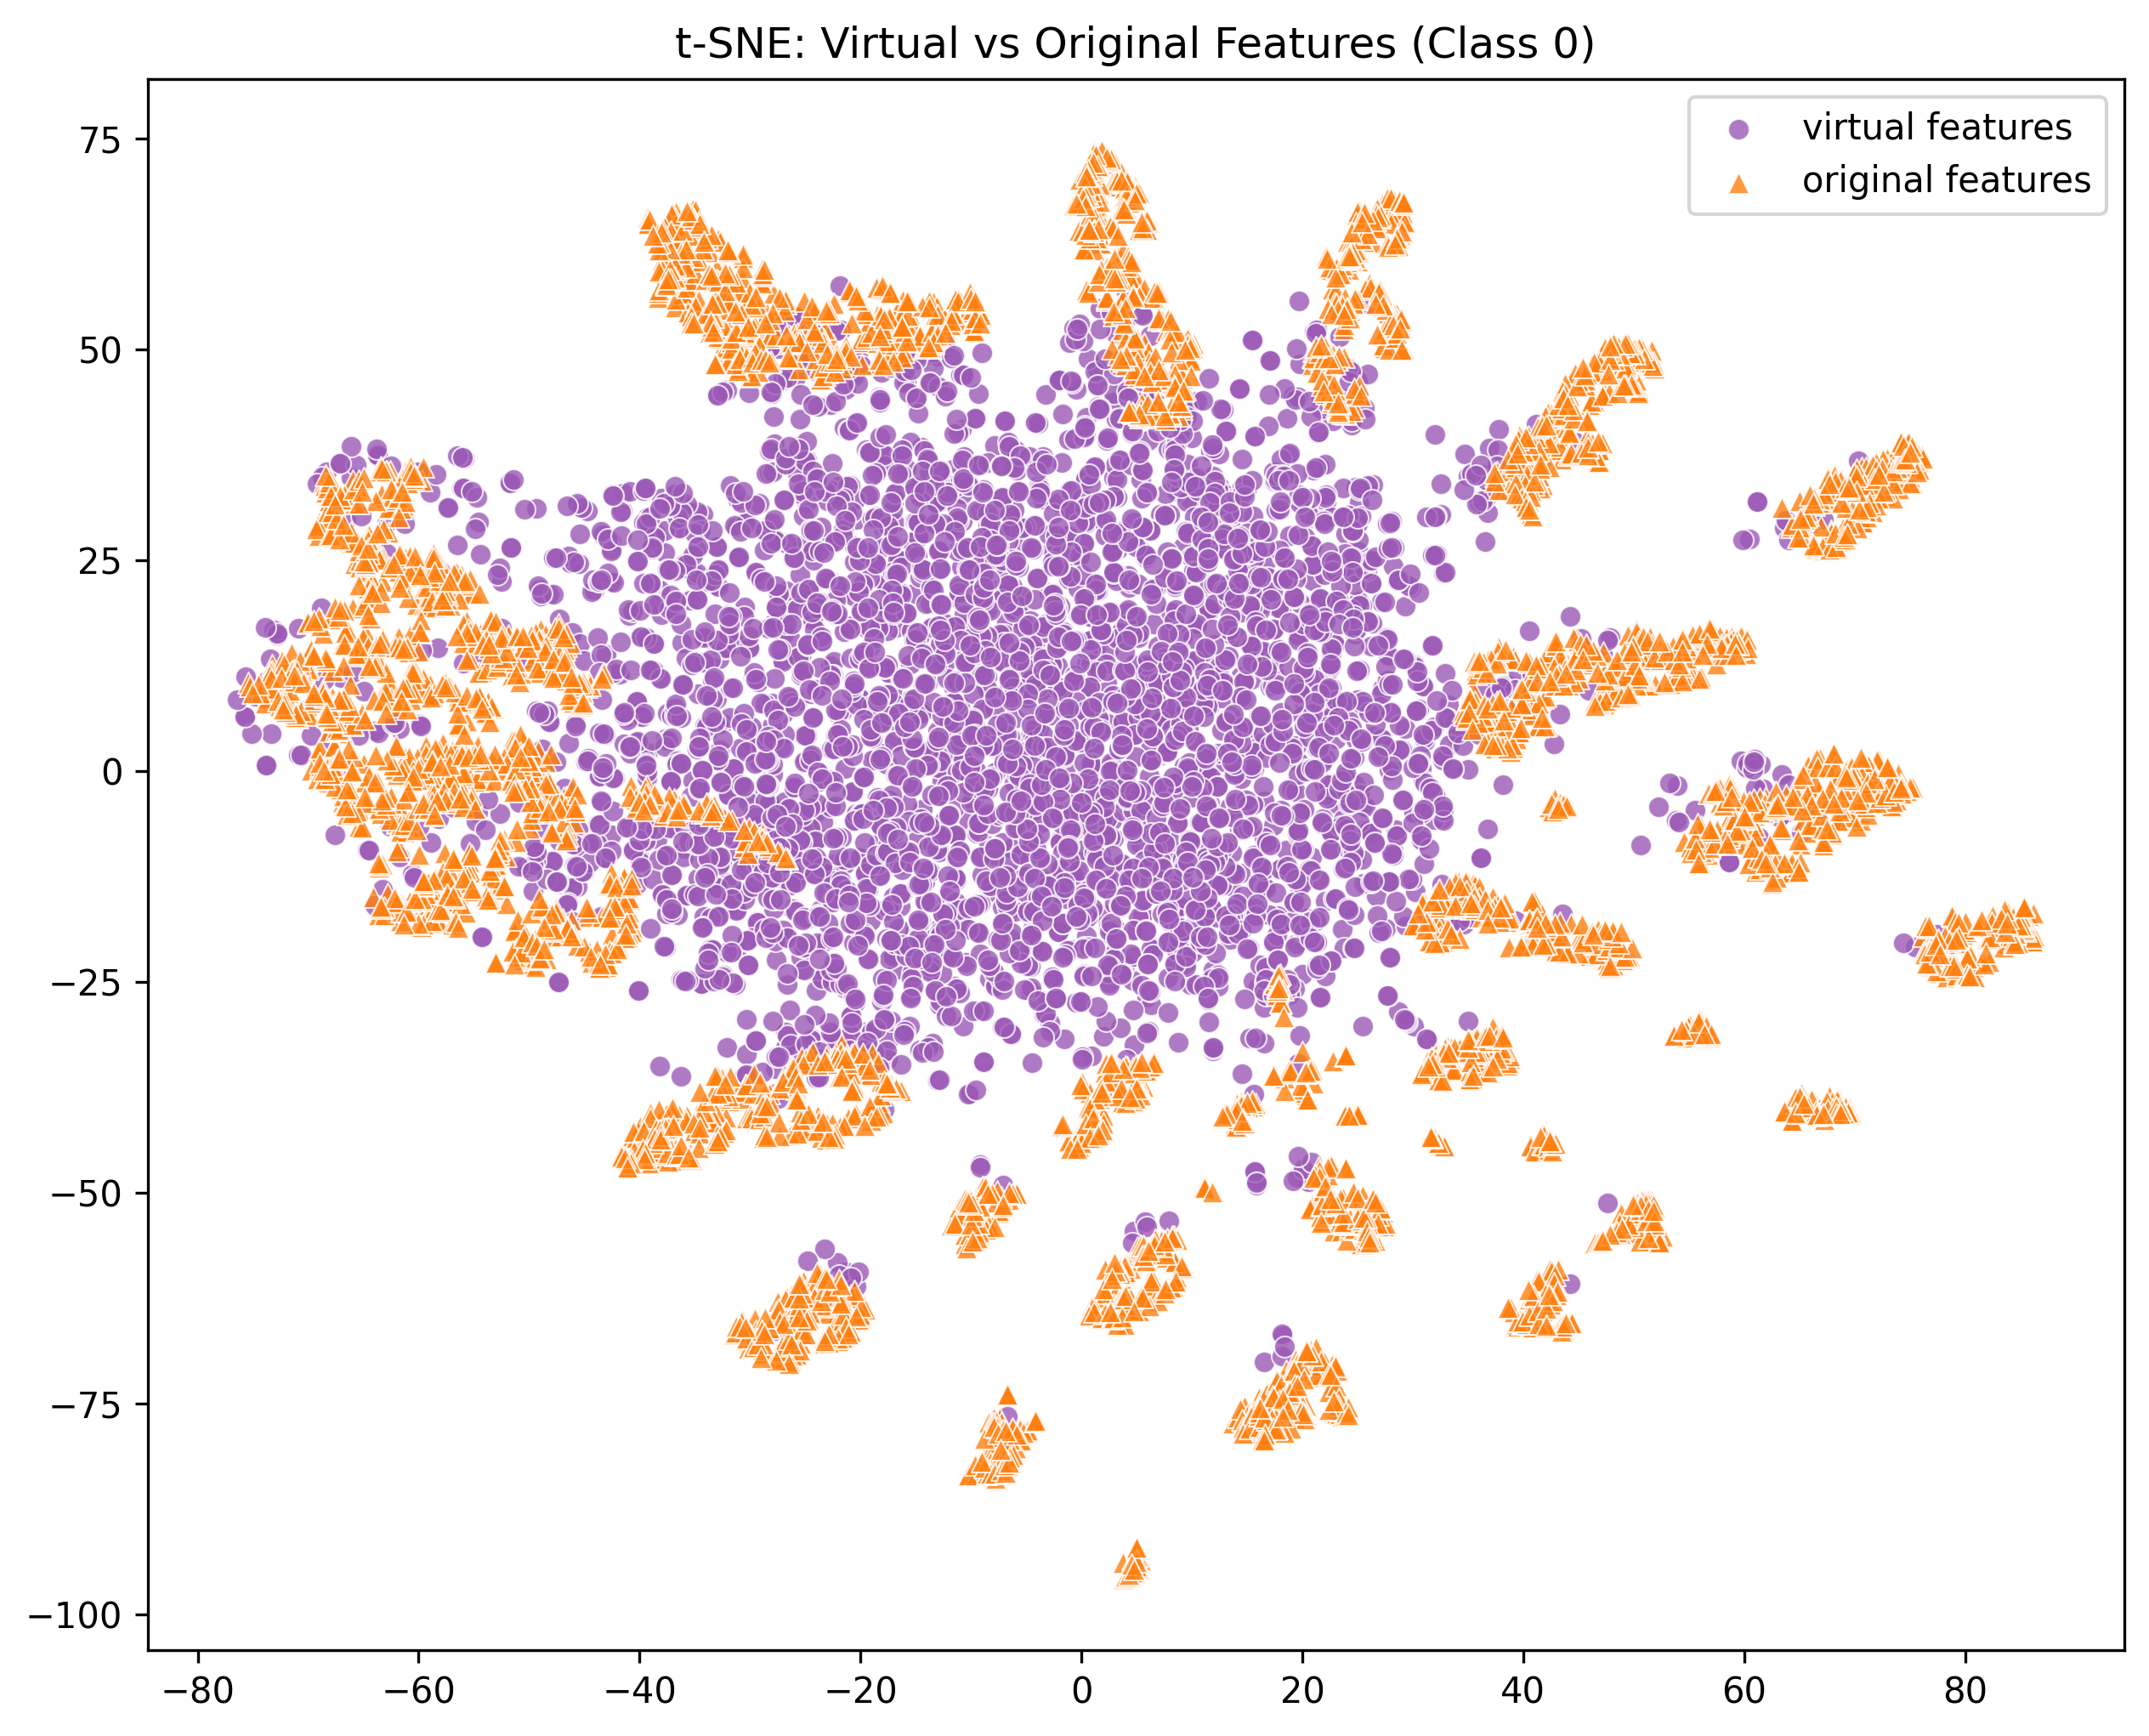
\includegraphics[width=0.8\linewidth]{imgs/tsne_class_0.png}
  \caption{After the first global round of training, the t-SNE visualization of virtual features and original features on FashionMNIST.}
  \label{tsne_class_0}
\end{figure}

\begin{figure*}[h]
    \centering
    \includegraphics[width=1\linewidth]{imgs/structure.png}
    \caption{General structure of the proposed semi-asynchronous energy-efficient federated prototype learning method}
    \label{fig:structure}
\end{figure*}

% \subsection{Details of Algorithm}

% The following is the algorithm.
\begin{breakablealgorithm}
  \caption{Semi-Asynchronous Energy-Efficient Federated Prototype learning for Client-Edge-Cloud Architectures}
  \begin{algorithmic}[1]
    % \State \textbf{Input: nothing}
    % \State \textbf{Output: nothing}

    \Procedure{cloud server executes}{}
    % \State Initialize global prototype set \( \bar{C}\) for all classes and weights for clients with heterogeneous models.
    \State Initialize weights for clients with heterogeneous models.
    \State All edge servers execute in parallel.
    \For{$t = 1, \dots, T$}
    \State Clear the buffer \(B\)

    \While{$B$ is not full} \Comment{Async process}
    \State Receive a triple \( (\mu^{l,edge}, \Sigma^{l,edge},\mathcal{N}^{l,edge}) \) from one edge server.
    \State Fill \( B \) with the received triple.
    \EndWhile
    \State \( \bar{C}, G \gets \text{CloudUpdate}(B) \)
    \State Send \( \bar{C}, G \) to edge servers participating on the current global aggregation.
    \State These edge servers re-execute.
    \EndFor
    \EndProcedure

    \Procedure{edge server executes}{}
    \State Receive \( \bar{C}, G \) from the cloud server
    \State Choose a set of clients $S^l$ to train in parallel.
    % \For{$e = 1, \dots, E$} \Comment{E now is static 1}
    \State Send \( \bar{C}, G \) to client \( i \in S^{l} \)
    \For{each client \( i \) in parallel}
    \State \( \textbf{ClientUpdate}(i, \bar{C}, G) \)
    \State Receive a triple \((\mu^{l,client}_i,\Sigma^{l,client}_i,\mathcal{N}^{l,client}_i)\)
    \EndFor \Comment{Wait for all clients}
    \State \( \textbf{EdgeAggregate}(\{ (\mu^{l,client}_i,\Sigma^{l,client}_i,\mathcal{N}^{l,client}_i) \}_{i \in S^{l}}) \)
    % \State \( \bar{C} \gets \text{EdgeUpdate}(\bar{C}, C^l) \) \Comment{not used now}
    % \EndFor
    \State Send a triple \( (\mu^{l,edge}, \Sigma^{l,edge},\mathcal{N}^{l,edge}) \) to the cloud server
    \EndProcedure
%   \end{algorithmic}
% \end{breakablealgorithm}

% % \newpage  % 强制换页

% \begin{breakablealgorithm}
%   \caption{Hierarchical Federated Prototype Learning -Part 2}
%   \begin{algorithmic}[1]
    \Procedure{CloudUpdate}{B}
    \State \( (\mu^{l,stored}, \Sigma^{l,stored},\mathcal{N}^{l,stored}) \gets (\mu^{l,edge}, \Sigma^{l,edge},\mathcal{N}^{l,edge})\quad\text{for}\quad l \in B \)
    \For{$j = 1, \dots, J$}
    \State \( \mathcal{N}_j = \sum_{l=1}^{L}\mathcal{N}^{l,stored}_{j} \)
    \State \( \text{Compute}\quad\mu_j,\Sigma_j\quad\text{by Eq.\ref{cloud mean},\ref{cloud covariance}}.  \)
    \EndFor
    \State Define $\mu$ as the global prototypes $\bar{C}$.
    \State Generate features \(X \sim \mathcal{N}(\mu, \Sigma)\) using the multivariate normal distribution.
    \State Use the virtual features \(X\) to train the global classifier \( G \).
    % \State Use adaptive-margin-enhanced contrastive learning to transform  $\bar{C}$ into $\bar{C}$
    \State \Return \( \bar{C}, G \)
    \EndProcedure
    
    \Procedure{EdgeAggregate}{$l, \{ (\mu^{l,client}_i, \Sigma^{l,client}_i,\mathcal{N}^{l,client}_i) \}_{i \in S^l}$}
    \State \( (\mu^{l,stored}_i, \Sigma^{l,stored}_i,\mathcal{N}^{l,stored}_i) \gets (\mu^{l,client}_i, \Sigma^{l,client}_i,\mathcal{N}^{l,client}_i)\quad\text{for}\quad i \in S^l \)
    \For{$j = 1, \dots, J$}
    \State \( \mathcal{N}^{l,edge}_j = \sum_{i=1}^{N^l}\mathcal{N}^{stored}_{i,j} \)
    \State \( \text{Compute}\quad\mu^{l,edge}_j,\Sigma^{l,edge}_j\quad\text{by Eq.\ref{edge mean},\ref{edge covariance}}.  \)
    \EndFor
    \State \Return \( (\mu^{l,edge}, \Sigma^{l,edge},\mathcal{N}^{l,edge}) \)
    \EndProcedure

    \Procedure{ClientUpdate}{$i, \bar{C}, G$}
    \State Receive \( \bar{C}, G \) from the edge server
    \State Only update one round and waiting for synchronization.
    \State Utilize the longest epoch training time to determine the operating frequency for subsequent $K-1$ rounds.
    \For{$k=1, \dots, K-1$}
    \State Scale the operating frequency.
    \For{batch (\(x,y\)) $\in$ \(D_i\)}
    \State Compute client prototypes by Eq.\ref{client prototype formula}.
    \State Compute loss by Eq.\ref{SAE loss function} using client prototypes and the global classifier $G$.
    \State Update client model according to the loss.
    \EndFor
    \EndFor
    \State Compute the mean $\mu^{l,client}_{i,j}$ and the covariance matrix  $\Sigma^{l,client}_{i,j}$ for features of each class 
    \Comment{Here, $\mu^{l,client}_{i,j}$ can be regarded as the prototype of class $j$ on the $i$-th client }
    \State \Return \( (\mu^{l,client}_i, \Sigma^{l,client}_i,\mathcal{N}^{l,client}_i) \)
    \EndProcedure
  \end{algorithmic}
\end{breakablealgorithm}

\section{Experiments}
\subsection{Setup}
\subsubsection{Datasets and algorithm implement}
We evaluate three popular benchmark datasets, including MNIST\cite{lecun1998mnist}, FashionMNIST\cite{xiao2017fashion}, and CIFAR-10\cite{krizhevsky2009learningcifar10}.  The client datasets are partitioned into training and testing sets in a 3:1 ratio.

For the implementation of the algorithm architecture, we extend the codebase of \cite{zhang2023pfllib}, adding a side for edge servers. In our settings, we simulate a cluster consisting of one cloud server, 10 edge servers, and 4 clients per edge server, with a consistently set client participation rate of 1. The number of local epochs is set to 5 and the number of global rounds is set to 200 for all experiments unless explicitly specified. To accelerate convergence and improve stability, we appropriately increase the batch size to 256, set the learning rate to 0.06, and configure the client training momentum of the SGD optimizer to 0.8.

For hyperparameter settings, we consistently set the importance weight $\lambda$ to 1, as reported in FedProto to achieve the highest test accuracy.  Additionally, we conduct comparative experiments by varying different $\gamma$ values. 
\subsubsection{Baselines}
We compared the proposed algorithm with several popular FL methods for heterogeneous models, including FedProto\cite{tan_fedproto_2021}, FedTGP\cite{zhang_fedtgp_2024}, FedGen\cite{zhu_data-free_fedgen_2021} , and  FedGH\cite{yi_fedgh_2023}.
\subsubsection{Statistical heterogeneity}
We conducted experiments following the practical statistical settings described in \cite{zhang_fedtgp_2024,li2021mode_moon}, and achieve the non-IID dataset partitioning using a Dirichlet distribution. Specifically, we sample \( q_j \sim Dir(\alpha) \) and allocate the proportion \( q_{i,j} \) of instances belonging to the class \( j \) to client \( i \), where \( Dir(\alpha) \) denotes a Dirichlet distribution with parameter \(\alpha\). This partitioning scheme allows each client to possess relatively more data samples in certain classes while having fewer or no samples in most other classes.
\subsubsection{Model heterogeneity}
We evaluate the model heterogeneity using eight distinct types of feature extractors, the same as in  \cite{zhang_fedtgp_2024}. For MNIST and FashionMNIST,  the model group includes eight distinct convolutional neural network architectures, which are composed of varying combinations of one or two convolutional layers, followed by pooling layers, and up to three fully connected layers with dimensions selected from 512 and 1024. For CIFAR-10, the model group is consistent with \cite{zhang_fedtgp_2024}, including 4-layer CNN, GoogleNet, MobileNet v2, ResNet18, ResNet34, ResNet50, ResNet101, and ResNet152.

\subsubsection{Environment}
Accuracy tests in Section \ref{Accuracy of Methods} are conducted using a machine equipped with 12 Intel(R) Xeon(R) Silver 4214R CPUs, an NVIDIA 3080 Ti GPU and Ubuntu 22.04 LTS.

As described in Section \ref{Energy-Efficient Training}, to validate the energy-saving performance in real-world computation-constrained environments, in Section \ref{Energy Efficiency Experiment} only FashionMNIST and MNIST are tested on NVIDIA Jetson TX2, which has a 6-core ARM CPU and 8GB DDR4 memory. The CPU frequency of Jetson TX2 range spans from 345,600 Hz to 2,035,200 Hz, with a total of 12 discrete frequency values. We utilize the interfaces provided in the NVIDIA documentation to monitor real-time power consumption and scale CPU frequencies.


\subsection{Accuracy of Methods}
\label{Accuracy of Methods}
As shown in the Table \ref{PC_test}, FedSAE achieves the best performance. In scenarios with high model heterogeneity and a large number of clients, improving accuracy is particularly challenging. During training, FedSAE not only brings difficult-to-classify samples closer to the global prototype but also makes the interclass distances more compact, as illustrated by Fig.\ref{exp_three_tsne}. FedProto shows a suboptimal clustering effect for prototypes, with the averaged prototypes of some clients exhibiting dispersed distributions that do not converge toward the global prototype. FedTGP effectively increases the interclass distance, and the prototype aggregation is better than that of FedProto, but its accuracy is lower.

To illustrate again, the hyperparameter $\gamma$ determines the contribution of the global classifier to the loss during local training. When $\gamma=1$, the global classifier completely replaces the local classifier for training. For MNIST and FashionMNIST, where client models are relatively simple, appropriately tuning the value of $\gamma$ can balance the contributions of global and local classifiers, thus improving training performance. For CIFAR-10, $\gamma=1$ achieves the best performance under various data distributions. We attribute this to the higher model complexity, where relying entirely on the global classifier during training enables more effective adaptation to diverse data distributions.

As shown in Fig.\ref{Cifar10_dir_03_Model_loss}, it can be observed that, except for FedTGP, the loss for other methods stabilizes as training converges. We follow the contrastive learning parameter settings for the cloud server as described in \cite{zhang_fedtgp_2024}, but FedTGP struggles to converge with a larger batch size, indicating that tuned hyperparameters may be necessary to achieve better performance. FedGH fails to train successfully on CIFAR-10. We suppose that this is due to the global classification head being trained solely on the averaged prototypes from clients, resulting in a significant mismatch between the local and global classification heads. Furthermore, the lack of regularization constraints for local training exacerbates this discrepancy, leading to a gradient explosion.


\begin{table*}[ht]
    \centering
    % \caption{The number of Edge servers is 10, 4 clients per edge server. Global rounds are set to 200, local epochs are set to 5, batchsize is 256, feature dimension is 512, local learning rate is 0.06, momentum is 0.8, \(\lambda\) is 1. Dirichlet distribution with a concentration parameter is $\alpha$. The buffer size of fedsae matches the number of edge servers.}
    \caption{The test accuracy on three datasets. The buffer size of FedSAE is equal to the number of edge servers.}
    \label{PC_test}
    \begin{tabular}{c c|c|c|c|c}
    \hline
    & & \multicolumn{2}{c|}{$\alpha = 0.1$}  & \multicolumn{2}{c}{$\alpha = 0.3$}\\
    \hline
    \textbf{Datasets} & \textbf{Methods} & \textbf{Prototype Acc(\%)} & \textbf{Model Acc(\%)} & \textbf{Prototype Acc(\%)} & \textbf{Model Acc(\%)} \\
    \hline
    \multirow{9}{*}{MNIST}
    & FedSAE($\gamma=1$) & \textbf{99.25} & 99.23 & 98.03 & 98.05  \\
    & FedSAE($\gamma=0.7$) & \textbf{99.25} & 99.23 & \textbf{98.08} & \textbf{98.08}  \\
    & FedSAE($\gamma=0.5$) & 99.24 & \textbf{99.24} & 98.04 & 98.06  \\
    & FedSAE($\gamma=0.2$) & 99.24 & 99.22 & 98.02 & 98.01  \\
    & Local Train & - & 98.97 & - & 97.31  \\
     & FedProto(AAAI'22) & 99.10 & 99.10 & 97.96 & 97.84 \\
     & FedTGP(AAAI'24) & 98.76 & 99.09 & 97.51 & 97.93 \\
     & FedGH(ACM MM'23) & - & 98.98 & - & 97.46 \\
     & FedGen(ICML'21) & - & 99.00 & - & 97.41 \\
    \hline
    \multirow{9}{*}{\makecell{Fashion\\ MNIST}} 
    & FedSAE($\gamma=1$) & 97.57 & 97.53 & 93.36 & 93.38 \\
    & FedSAE($\gamma=0.7$) & \textbf{97.62} & 97.55 & 93.30 & 93.41  \\
    & FedSAE($\gamma=0.5$) & 97.54 & \textbf{97.56} & \textbf{93.41} & \textbf{93.42}  \\
    & FedSAE($\gamma=0.2$) & 97.54  & 97.55 & 93.27 & 93.39  \\
    & Local Train & - & 97.15 & - & 92.56  \\
     & FedProto(AAAI'22) & 97.48 & 97.47 & 93.10 & 93.13 \\
     & FedTGP(AAAI'24) & \ding{55} & \ding{55} & \ding{55} & \ding{55} \\
     & FedGH(ACM MM'23) & - & 97.21(\ding{55}) & - & 92.51 \\
     & FedGen(ICML'21) & - & 97.34& - & 92.63\\
    \hline
    \multirow{9}{*}{CIFAR-10} 
    & FedSAE($\gamma=1$) & \textbf{82.06} & \textbf{82.08} & \textbf{67.27} & 67.22 \\
    & FedSAE($\gamma=0.7$) & 81.81 & 81.92 & 67.24 & \textbf{67.23} \\
    & FedSAE($\gamma=0.5$) & 81.62 & 81.60 & 67.11 & 67.01 \\
    & FedSAE($\gamma=0.2$) & 81.60 & 81.68 & 66.57 & 66.49 \\
    & Local Train & - & 81.06 & - & 65.97 \\
     & FedProto(AAAI'22) & 81.04 & 81.88 & 66.13 & 66.32 \\
     & FedTGP(AAAI'24) & 79.92 & 80.96 & 66.27 & 66.07 \\
     & FedGH(ACM MM'23) & - & \ding{55} & - & \ding{55} \\
     & FedGen(ICML'21) & - & 81.72 & - & 65.85\\
    \hline
    \end{tabular}
\end{table*}

\begin{figure}[htbp]
    \centering
    \includegraphics[width=0.96\linewidth]{imgs/Cifar10_dir_03_Model_loss.png}
    \caption{The training loss on CIFAR-10 with $\alpha=0.3$}
    \label{Cifar10_dir_03_Model_loss}
\end{figure}

\begin{figure*}[htbp]
    \centering
    % 子图1
    \subfloat[FedProto]{%
        \includegraphics[width=0.3\linewidth]{imgs/FedProto_tsne_agg_epoch_200_fd512.png}
        \label{FedProto_tsne_agg_epoch_200_fd512}
    }
    % 子图2
    \subfloat[FedSAE($\gamma=1$)]{%
        \includegraphics[width=0.3\textwidth]{imgs/FedSAE_gamma1_bf10_tsne_agg_epoch_200_fd512.png}
        \label{FedSAE_gamma1_bf10_tsne_agg_epoch_200_fd512}
    }
    \subfloat[FedTGP]{%
        \includegraphics[width=0.3\linewidth]{imgs/FedTGP_tsne_agg_epoch_200_fd512.png}
        \label{FedTGP_tsne_agg_epoch_200_fd512}
    }

    \caption{After 200 global rounds, the t-SNE visualization of aggregated prototypes generated by different methods on CIFAR-10. The experimental settings is consistent with Table \ref{PC_test}, and Dirichlet distribution parameter $\alpha=0.3$.}
    \label{exp_three_tsne}
\end{figure*}

\subsection{Impact of Feature Dimensions}
\label{Impact of Feature Dimensions}

As shown in Table \ref{different Dims table}, we evaluated the performance of various methods on CIFAR-10 using different feature dimensions. FedSAE outperforms FedProto in both low-dimensional and high-dimensional settings. However, FedProto surpasses FedSAE when the feature dimension is 256. Although FedTGP achieves the best performance at \( \kappa = 64 \) and \( \kappa = 256 \), as mentioned in the previous section, its convergence cannot be guaranteed.


\begin{table}[ht]
    \centering
    \caption{Test accuracies(\%) on CIFAR-10 with different feature dimensions. The number of Edge servers is 10, 4 clients per edge server. the $\gamma$ of FedSAE is 1.}
    \begin{tabular}{|c|c|c|c|c|}
    \hline
    \textbf{Methods} & $\kappa$=64  & $\kappa$=256 & $\kappa$=1024 \\
    \hline
    Local Train & 66.16 & 66.33 & 65.31 \\
    FedSAE & 67.24/67.40 & 66.87/66.95 & \textbf{65.73/65.68} \\
    FedProto & 66.90/67.00 & 67.27/67.17 & 64.96/65.13 \\
    FedTGP & \textbf{67.83/67.47} & \textbf{67.45/67.23} & 64.30/65.20\\
    % FedGH &  &  & \\
    FedGen & 66.68 & 66.53 & 65.55 \\
    \hline
    \end{tabular}
    \label{different Dims table}
\end{table}


\subsection{Energy Efficiency Experiment}
\label{Energy Efficiency Experiment}
The size of the covariance matrix is proportional to the square of the dimension of the feature vectors. To reduce communication overhead, the dimension of the feature vectors is set to 64. The communication time is calculated using Shannon's formula\cite{shannon1948mathematical}. The time required for a local client to upload data to an edge server can be expressed by formula $T_{\text{com}} = \frac{W}{B\cdot\log_2\left(1 + \frac{h\cdot p}{N_0}\right)}$. Following the experimental setup in \cite{liu_hierarchical_2023}, $W$ represents the size of the data uploaded in bits, $B = 1 \times 10^6$ Hz is the channel bandwidth, $h = 10^{-8}$ is the channel gain, $p = 0.5$ W is the transmission power and $N_0 = 10^{-10}$ W is the noise power. The communication time between the edge server and the cloud server is assumed to be 10 times that between the clients and the edge server.

Specifically, for a feature vector with a dimension of 512, where each single-precision floating-point number occupies 4 bytes, the size is approximately 2 KB. When the client uploads 10 categories of average prototypes, the total transmission size is 20 KB, resulting in a theoretical communication time of 0.029 seconds for FedProto, which can be considered negligible. 

In contrast, for FedSAE, in addition to the average prototypes, the covariance matrix for all categories occupies about 10 MB, leading to a theoretical communication time of 14.8 seconds. To reduce the communication overhead of FedSAE, the dimension of features is set to 64, decreasing the communication time to 0.235 seconds. The global classifier's weights are very small, totaling only 4 KB, so the communication time between the edge and the cloud is approximately 2.35 seconds.

We first run a long-duration FedProto experiment on the Jetson TX2, collecting its energy consumption and runtime data. As shown in Fig.\ref{100rounds_with_fit_and_R2}, it can be observed that when training is performed on the CPU, both runtime and power consumption increase linearly. To enable a more intuitive comparison, we evaluate the metrics for each parameter setting at a specific midpoint, under the same global time conditions. The final accuracy is shown in Table \ref{DVFS_experiment}, with the edge server participating in a total of 1000 updates.

\begin{figure}
  \centering
  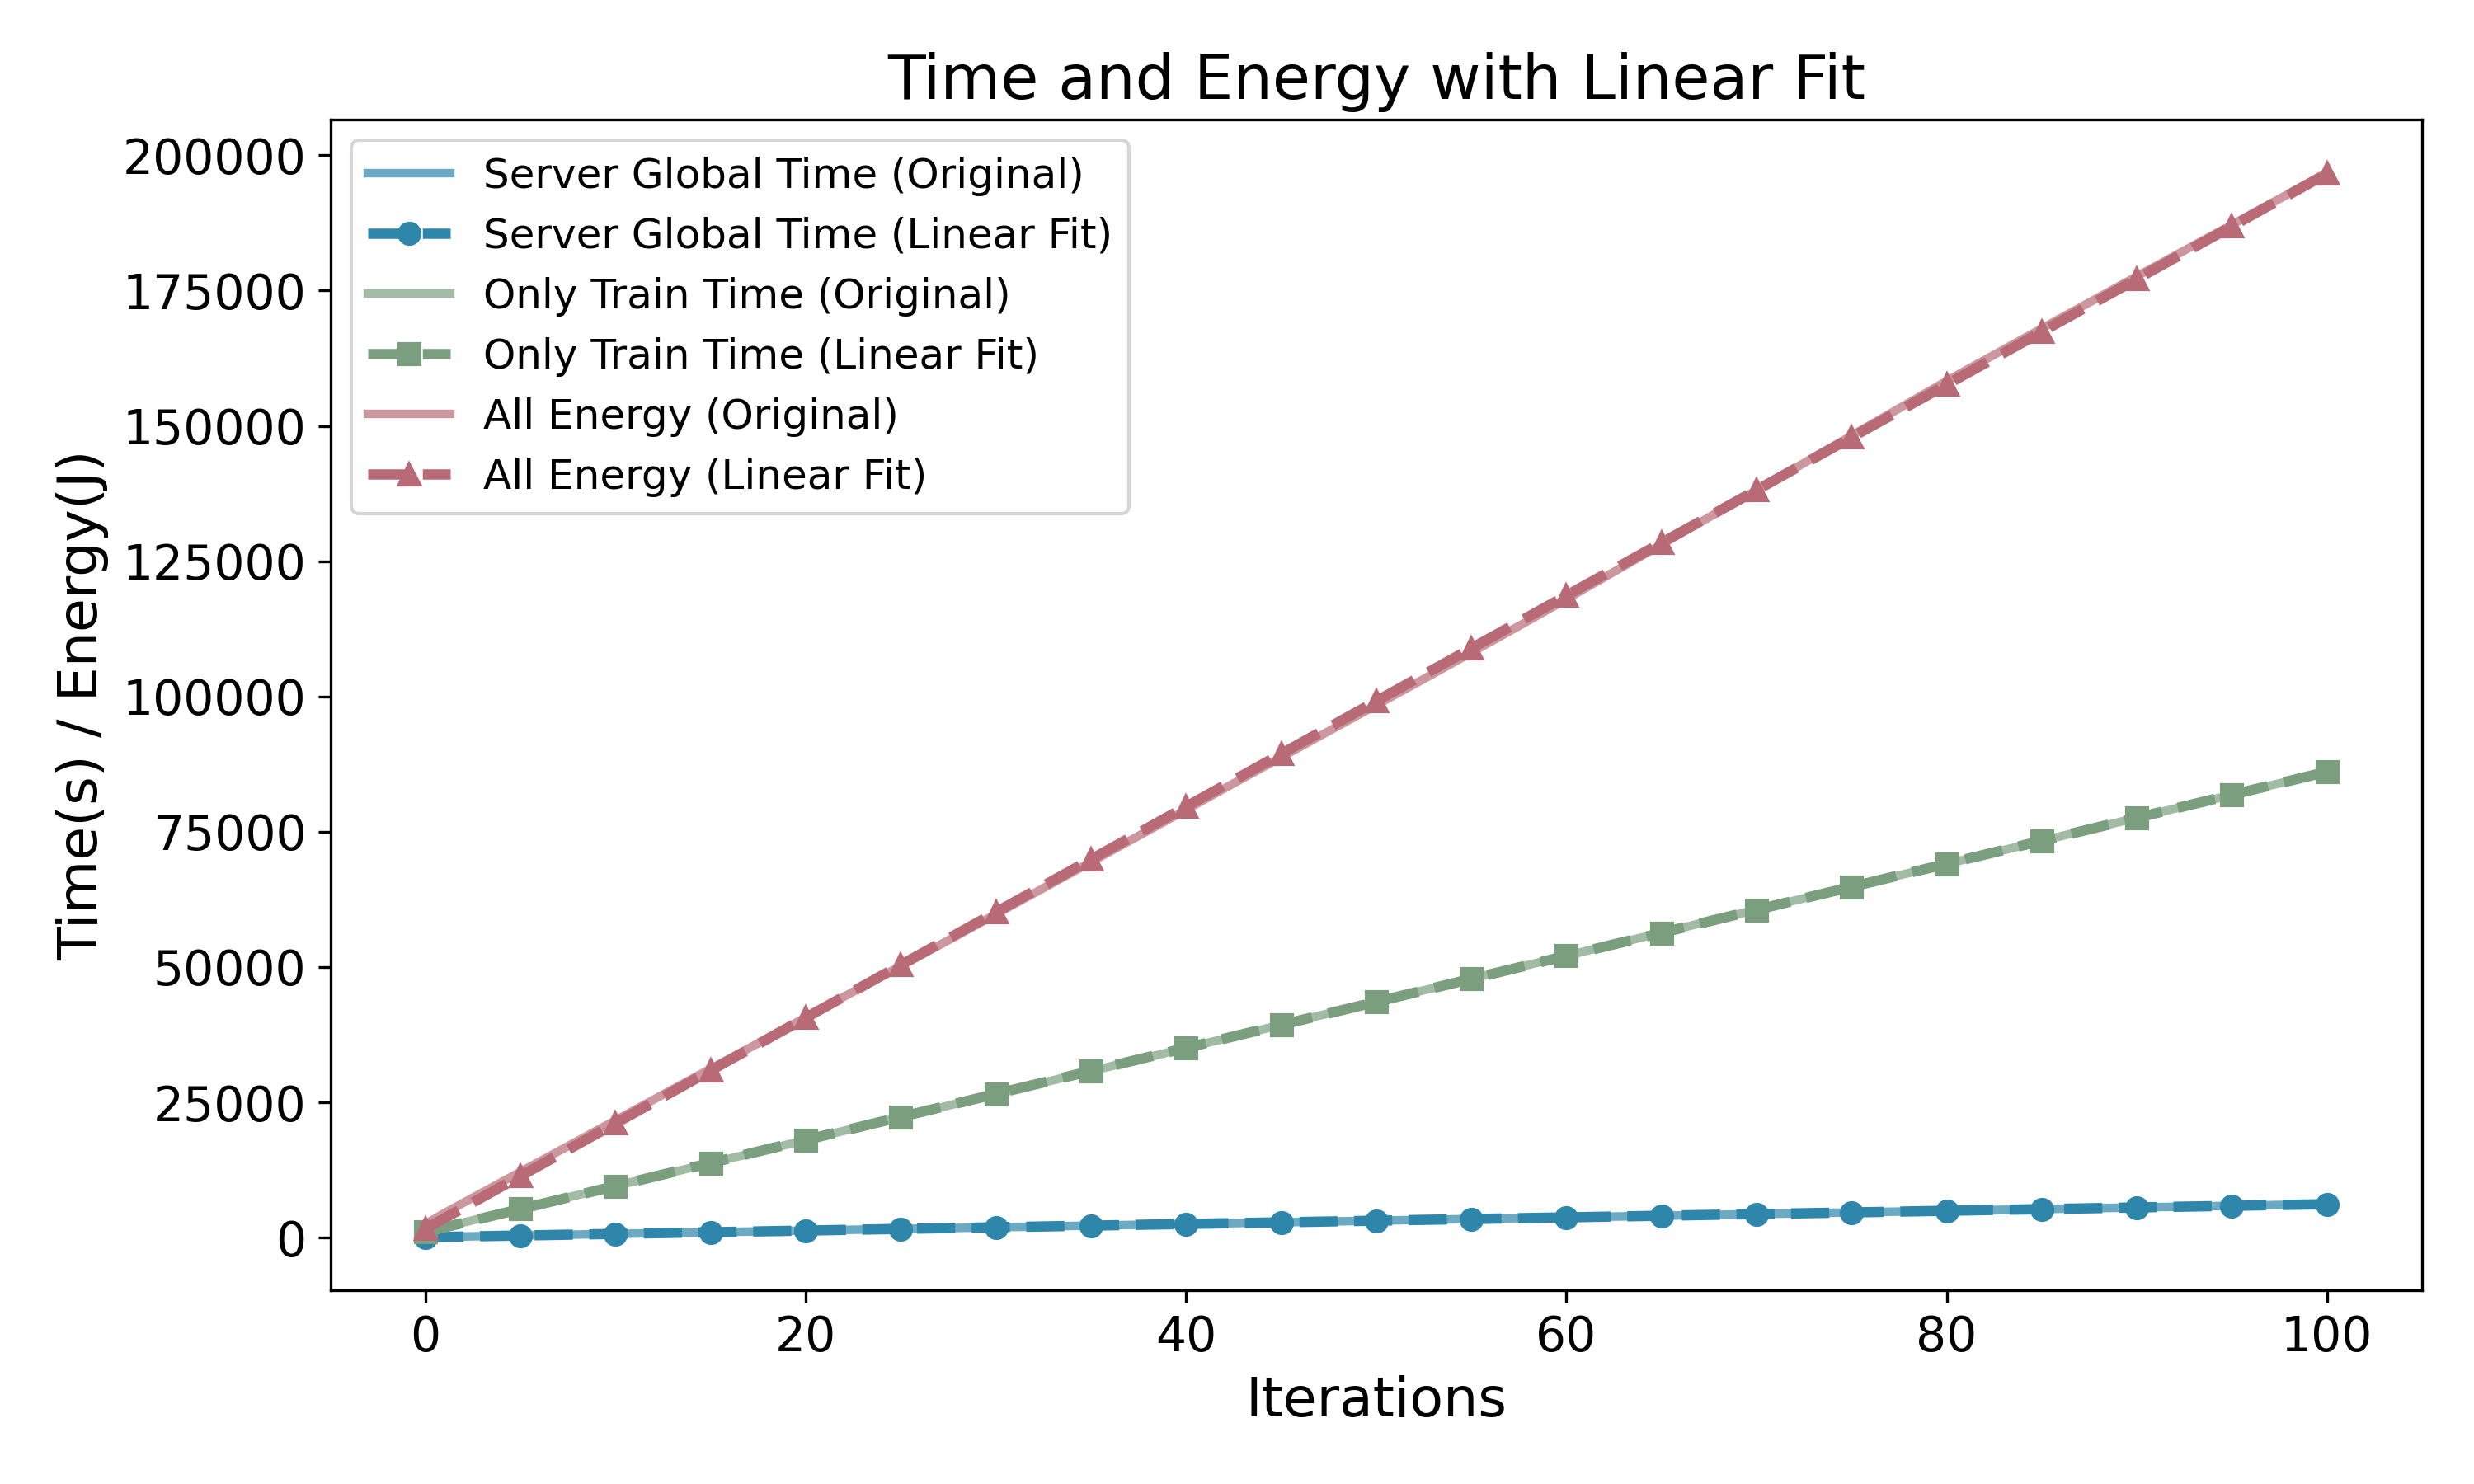
\includegraphics[width=0.9\linewidth]{imgs/100rounds_with_fit_and_R2.png}
  \caption{Train 100 rounds of FedProto on FashionMNIST on Jetson TX2. 10 edges with 4 clients per edge server. The local epochs is 3 and $\alpha$ is 0.3, other experimental settings are consistent with Section \ref{Accuracy of Methods}.}
  \label{100rounds_with_fit_and_R2}
\end{figure}


\begin{table*}[ht]
    \centering
    \caption{Local epochs is 3 and Dirichlet distribution parameter $\alpha$ is 0.3. Other Experimental Settings is Consistent with Table \ref{PC_test}. The buffer size (BS) of FedSAE is selected from $\{1, 3, 5, 10\}$. }
    \begin{tabular}{|c|c|c|c|c|c|c|c|c|}
    \hline
    \textbf{Datasets} & \textbf{Methods} & \textbf{\makecell{Global\\Time(s)}} & \textbf{\makecell{Train\\Time(s)}} & \textbf{\makecell{Prototype\\Acc(\%)}} & \textbf{\makecell{Model\\Acc(\%)}} &\textbf{Energy (kJ)} & \textbf{\makecell{Final prototype\\Acc(\%)}} & \textbf{\makecell{Final model\\Acc(\%)}}\\  
    \hline
    \multirow{6}{*}{MNIST} 
    & FedSAE($BS=10$) & \multirow{6}{*}{\makecell{1200}} &  &  &  &  &  & \\
    & FedSAE($BS=5$) &  &  &  &  &  &  & \\
    & FedSAE($BS=3$) &  &  &  &  &  &  & \\
    & FedSAE($BS=1$) &  &  &  &  &  &  & \\
    % & Local Train &  &  &  &  &  &  & \\
    & FedProto &  &  &  &  &  &  & \\
    & FedProto + DVFS &  &  &  &  &  &  & \\
    \hline
    \multirow{6}{*}{\makecell{Fashion\\ MNIST}} 
    & FedSAE($BS=10$) & \multirow{6}{*}{\makecell{1200}} &  &  &  &  & 93.21 & 93.22\\
    & FedSAE($BS=5$) &  &  &  &  &  & 93.33 & 93.28 \\
    & FedSAE($BS=3$) &  &  &  &  &  & 93.25 & 93.28\\
    & FedSAE($BS=1$) &  &  &  &  &  & 93.10 & 93.15 \\
    % & Local Train &  &  &  &  &  &  & \\
    & FedProto &  & 15806 & 89.69 & 91.41 & 3.6877 & 93.00 & 93.01\\
    & FedProto + DVFS &  &  &  &  &  &  & \\
    \hline
    \end{tabular}
    \label{DVFS_experiment}
\end{table*}



% \subsection{Communication Cost}



\section{Conclusion}


% use section* for acknowledgment
\section*{Acknowledgment}

This work was supported in part by the National Natural Science Foundation of China under Grant No.62302323, 62172061 and U2268204; National Key R\&D Program of China under Grant No. 2023YFB3308300; DEC-SCU Joint Innovation Research Institute Project No.23H0643.
\bibliography{SAE} 
\bibliographystyle{IEEEtran}


\appendices
\onecolumn

\section{Derivation of both Global Mean and Covariance}
\(k\) is the \(k\)-th client, \(l\) is the \(l\)-th edge server, \(c\) is the \(c\)-th class. \( N(c,k,l) \) is the number of samples of class \( c \) in the client \( k \) on the edge server \( l \). \( N(c,l) \) is the number of samples of class \( c \) in the edge server \( l \). \( N(c) \) is the number of samples of class \( c \) at the cloud server.

Mean and covariance of client:
\begin{equation}
\mathbf{\mu}_{c,k,l} = \frac{1}{N(c,k,l)} \sum_{i=1}^{N(c,k,l)} \mathbf{x}_{i,c,k,l}
\end{equation}
\begin{equation}
\mathbf{\Sigma}_{c,k,l} = \frac{1}{N(c,k,l)-1} \sum_{i=1}^{N(c,k,l)} \big( \mathbf{x}_{i,c,k,l} - \mathbf{\mu}_{c,k,l} \big) \big( \mathbf{x}_{i,c,k,l} - \mathbf{\mu}_{c,k,l} \big)^\top,
\end{equation}

Mean and covariance of edge:
\begin{equation}
  N(c,l) = \sum_{k=1}^K N(c,k,l).
\end{equation}
\begin{equation}
    \mathbf{\mu}_{c,l} = \frac{1}{N(c,l)} \sum_{k=1}^K N(c,k,l) \mathbf{\mu}_{c,k,l},
    \end{equation}
\begin{equation}
\mathbf{\Sigma}_{c,l} = \frac{1}{N(c,l)-1} \sum_{k=1}^K \Bigg[
\big( N(c,k,l)-1 \big) \mathbf{\Sigma}_{c,k,l} + N(c,k,l) \big( \mathbf{\mu}_{c,k,l} - \mathbf{\mu}_{c,l} \big) \big( \mathbf{\mu}_{c,k,l} - \mathbf{\mu}_{c,l} \big)^\top
\Bigg],
\end{equation}

Derivation of edge covariance:

Consider \( \mathbf{z}_{i,c,k,l} = \mathbf{x}_{i,c,k,l} - \mathbf{\mu}_{c,k,l} \) as the deviation of the sample from the local mean at the client \(k \). And \(\sum_{i=1}^{N(c,k,l)} \mathbf{z}_{i,c,k,l} = 0  \)

\begin{align*}
  \mathbf{\Sigma}_{c,l} &= \frac{1}{N(c,l)-1} \sum_{k=1}^K \sum_{i=1}^{N(c,k,l)} \big( \mathbf{x}_{i,c,k,l} - \mathbf{\mu}_{c,l} \big) \big( \mathbf{x}_{i,c,k,l} - \mathbf{\mu}_{c,l} \big)^\top \\
  &= \frac{1}{N(c,l)-1} \sum_{k=1}^K \sum_{i=1}^{N(c,k,l)} \left( \big( \mathbf{\mu}_{c,k,l} + \mathbf{z}_{i,c,k,l} - \mathbf{\mu}_{c,l} \big) \big( \mathbf{\mu}_{c,k,l} + \mathbf{z}_{i,c,k,l} - \mathbf{\mu}_{c,l} \big)^\top \right) \\
  &= \frac{1}{N(c,l)-1} \sum_{k=1}^K \sum_{i=1}^{N(c,k,l)} \Bigg[ \big( \mathbf{\mu}_{c,k,l} - \mathbf{\mu}_{c,l} \big) \big( \mathbf{\mu}_{c,k,l} - \mathbf{\mu}_{c,l} \big)^\top \\
  &\quad + \mathbf{z}_{i,c,k,l} \mathbf{z}_{i,c,k,l}^\top + \big( \mathbf{\mu}_{c,k,l} - \mathbf{\mu}_{c,l} \big) \mathbf{z}_{i,c,k,l}^\top + \mathbf{z}_{i,c,k,l} \big( \mathbf{\mu}_{c,k,l} - \mathbf{\mu}_{c,l} \big)^\top \Bigg] \\
  &= \frac{1}{N(c,l)-1} \sum_{k=1}^K \Bigg[ (N(c,k,l)-1) \mathbf{\Sigma}_{c,k,l} + N(c,k,l) \big( \mathbf{\mu}_{c,k,l} - \mathbf{\mu}_{c,l} \big) \big( \mathbf{\mu}_{c,k,l} - \mathbf{\mu}_{c,l} \big)^\top \Bigg]
\end{align*}

Mean and covariance of cloud:

First, use the decomposition:
\begin{equation}
\mathbf{x}_{i,c,k,l} - \mathbf{\mu}_c = \big( \mathbf{x}_{i,c,k,l} - \mathbf{\mu}_{c,l} \big) + \big( \mathbf{\mu}_{c,l} - \mathbf{\mu}_c \big),
\end{equation}

We substitute into the covariance definition:
\begin{align*}
\mathbf{\Sigma}_c 
&= \frac{1}{N(c)-1} \sum_{l=1}^L \sum_{k=1}^K \sum_{i=1}^{N(c,k,l)} 
\big( \mathbf{x}_{i,c,k,l} - \mathbf{\mu}_c \big) \nonumber \times 
\big( \mathbf{x}_{i,c,k,l} - \mathbf{\mu}_c \big)^\top \\ 
&= \frac{1}{N(c)-1} \sum_{l=1}^L \sum_{k=1}^K \sum_{i=1}^{N(c,k,l)} 
\Big[
\big( \mathbf{x}_{i,c,k,l} - \mathbf{\mu}_{c,l} \big) + \big( \mathbf{\mu}_{c,l} - \mathbf{\mu}_c \big)
\Big] \nonumber \\
&\qquad \times 
\Big[
\big( \mathbf{x}_{i,c,k,l} - \mathbf{\mu}_{c,l} \big) + \big( \mathbf{\mu}_{c,l} - \mathbf{\mu}_c \big)
\Big]^\top.
\end{align*}

Expanding the terms:
\begin{align}
\mathbf{\Sigma}_c &= \frac{1}{N(c)-1} \sum_{l=1}^L \sum_{k=1}^K \sum_{i=1}^{N(c,k,l)} 
\Big[
\mathbf{Z}_{i,c,k,l} \mathbf{Z}_{i,c,k,l}^\top + 
\mathbf{Z}_{i,c,k,l} \big( \mathbf{\mu}_{c,l} - \mathbf{\mu}_c \big)^\top \nonumber \\
&\qquad + 
\big( \mathbf{\mu}_{c,l} - \mathbf{\mu}_c \big) \mathbf{Z}_{i,c,k,l}^\top + 
\big( \mathbf{\mu}_{c,l} - \mathbf{\mu}_c \big) \big( \mathbf{\mu}_{c,l} - \mathbf{\mu}_c \big)^\top
\Big].
\end{align}

Here, \( \mathbf{Z}_{i,c,k,l} = \mathbf{x}_{i,c,k,l} - \mathbf{\mu}_{c,l} \) represents the deviation of local samples from their respective edge means.

Simplification of Cross Terms
The cross terms are:
\begin{equation}
\mathbf{Z}_{i,c,k,l} \big( \mathbf{\mu}_{c,l} - \mathbf{\mu}_c \big)^\top, \quad
\big( \mathbf{\mu}_{c,l} - \mathbf{\mu}_c \big) \mathbf{Z}_{i,c,k,l}^\top.
\end{equation}

Summing over all samples, these terms vanish because:
\begin{equation}
  \sum_{k=1}^K \sum_{i=1}^{N(c,k,l)} \mathbf{Z}_{i,c,k,l} = \mathbf{0}
\end{equation}

Consider the summation of deviations for client \( k \) at edge \( l \):
\begin{align*}
\sum_{k=1}^K\sum_{i=1}^{N(c,k,l)} \mathbf{Z}_{i,c,k,l} &= \sum_{k=1}^K \sum_{i=1}^{N(c,k,l)} \big( \mathbf{x}_{i,c,k,l} - \mathbf{\mu}_{c,l} \big) \\
&= \sum_{k=1}^K\sum_{i=1}^{N(c,k,l)} \mathbf{x}_{i,c,k,l} - \sum_{k=1}^K\sum_{i=1}^{N(c,k,l)} \mathbf{\mu}_{c,l}. \\
&= \sum_{k=1}^K\sum_{i=1}^{N(c,k,l)} \mathbf{x}_{i,c,k,l} - \sum_{k=1}^K N(c,k,l) \mathbf{\mu}_{c,l} \\
&= \sum_{k=1}^K\sum_{i=1}^{N(c,k,l)} \mathbf{x}_{i,c,k,l} - \sum_{k=1}^K\frac{N(c,k,l)}{N(c,l)} \sum_{k=1}^K \sum_{i=1}^{N(c,k,l)} \mathbf{x}_{i,c,k,l} \\
&= 0
\end{align*}



Final Formula
The cloud-level covariance reduces to:
\begin{align}
\mathbf{\Sigma}_c &= \frac{1}{N(c)-1} \Bigg[
\sum_{l=1}^L \sum_{k=1}^K \sum_{i=1}^{N(c,k,l)} \mathbf{Z}_{i,c,k,l} \mathbf{Z}_{i,c,k,l}^\top + 
\sum_{l=1}^L N(c,l) \big( \mathbf{\mu}_{c,l} - \mathbf{\mu}_c \big) \big( \mathbf{\mu}_{c,l} - \mathbf{\mu}_c \big)^\top
\Bigg] \nonumber \\
&= \frac{1}{N(c)-1} \Bigg[
\sum_{l=1}^L (N(c,l)-1) \mathbf{\Sigma}_{c,l} + 
\sum_{l=1}^L N(c,l) \big( \mathbf{\mu}_{c,l} - \mathbf{\mu}_c \big) \big( \mathbf{\mu}_{c,l} - \mathbf{\mu}_c \big)^\top
\Bigg].
\end{align}


\section{Features of test dataset}

\begin{figure*}[htbp]
    \centering
    % % 子图1
    % \subfloat[Average Prototypes of FedSAE($\gamma$=1)]{%
    %     \includegraphics[width=0.45\linewidth]{imgs/test_umap_FedSAE_visualization_protos.png}
    %     \label{test_umap_FedSAE_visualization_protos}
    % }
    % % \hfill
    % % 子图2
    % \subfloat[Average Prototypes of  FedProto]{%
    %     \includegraphics[width=0.45\linewidth]{imgs/test_umap_FedSAE_visualization_protos.png}
    %     \label{test_umap_FedSAE_visualization_protos}
    % }


    \subfloat[Features of FedSAE($\gamma$=1)]{%
        \includegraphics[width=0.45\linewidth]{imgs/onlytrue_umap_FedSAE_visualization.png}
        \label{onlytrue_umap_FedSAE_visualization}
    }
    % \hfill
    % 子图2
    \subfloat[Features of FedProto]{%
        \includegraphics[width=0.45\linewidth]{imgs/onlytrue_umap_FedProto_visualization.png}
        \label{onlytrue_umap_FedProto_visualization}
    }

    \caption{After 200 global rounds, the UMAP visualization\cite{mcinnes2018umap-software} of features of correctly classified samples on CIFAR-10 where $\alpha$=0.1, local train epochs is 5, and the dimension of hidden features (prototypes) is 512.}
    \label{UMAP}
\end{figure*}

\end{document}


